\documentclass[a4paper,10pt,twocolumn,oneside]{article}
\setlength{\columnsep}{10pt}                                                                    %兩欄模式的間距
\setlength{\columnseprule}{0pt}                                                                %兩欄模式間格線粗細

\usepackage{amsthm}								%定義,例題
\usepackage{amssymb}
%\usepackage[margin=2cm]{geometry}
\usepackage{fontspec}								%設定字體
\usepackage{color}
\usepackage[x11names]{xcolor}
\usepackage{xeCJK}								%xeCJK
\usepackage{listings}								%顯示code用的
%\usepackage[Glenn]{fncychap}						%排版,頁面模板
\usepackage{fancyhdr}								%設定頁首頁尾
\usepackage{graphicx}								%Graphic
\usepackage{enumerate}
\usepackage{titlesec}
\usepackage{amsmath}
\usepackage{pdfpages}
%\usepackage[T1]{fontenc}
\usepackage{amsmath, courier, listings, fancyhdr, graphicx}
\topmargin=0pt
\headsep=5pt
\textheight=780pt
\footskip=0pt
\voffset=-40pt
\textwidth=545pt
\marginparsep=0pt
\marginparwidth=0pt
\marginparpush=0pt
\oddsidemargin=0pt
\evensidemargin=0pt
\hoffset=-42pt

%\renewcommand\listfigurename{圖目錄}
%\renewcommand\listtablename{表目錄} 

%%%%%%%%%%%%%%%%%%%%%%%%%%%%%

%\setmainfont{Consolas}				%主要字型
%\setmainfont{Linux Libertine G}
\setmonofont{Consolas}
%B\setCJKmainfont{Source Han Sans}			%中文字型
%\setmainfont{sourcecodepro}
\XeTeXlinebreaklocale "zh"						%中文自動換行
\XeTeXlinebreakskip = 0pt plus 1pt				%設定段落之間的距離
\setcounter{secnumdepth}{3}						%目錄顯示第三層

%%%%%%%%%%%%%%%%%%%%%%%%%%%%%
\makeatletter
\lst@CCPutMacro\lst@ProcessOther {"2D}{\lst@ttfamily{-{}}{-{}}}
\@empty\z@\@empty
\makeatother
\lstset{											% Code顯示
language=C++,										% the language of the code
basicstyle=\footnotesize\ttfamily, 						% the size of the fonts that are used for the code
%numbers=left,										% where to put the line-numbers
numberstyle=\footnotesize,						% the size of the fonts that are used for the line-numbers
stepnumber=1,										% the step between two line-numbers. If it's 1, each line  will be numbered
numbersep=5pt,										% how far the line-numbers are from the code
backgroundcolor=\color{white},					% choose the background color. You must add \usepackage{color}
showspaces=false,									% show spaces adding particular underscores
showstringspaces=false,							% underline spaces within strings
showtabs=false,									% show tabs within strings adding particular underscores
frame=false,											% adds a frame around the code
tabsize=2,											% sets default tabsize to 2 spaces
captionpos=b,										% sets the caption-position to bottom
breaklines=true,									% sets automatic line breaking
breakatwhitespace=false,							% sets if automatic breaks should only happen at whitespace
escapeinside={\%*}{*)},							% if you want to add a comment within your code
morekeywords={*},									% if you want to add more keywords to the set
keywordstyle=\bfseries\color{Blue1},
commentstyle=\itshape\color{Red4},
stringstyle=\itshape\color{Green4},
}

%%%%%%%%%%%%%%%%%%%%%%%%%%%%%

\def\footnotesize{\fontsize{8}{9}\selectfont}

\begin{document}
\pagestyle{fancy}
\fancyfoot{}
%\fancyfoot[R]{\includegraphics[width=20pt]{ironwood.jpg}}
\fancyhead[L]{nWa}
\fancyhead[R]{\thepage}
\renewcommand{\headrulewidth}{0.4pt}
\renewcommand{\contentsname}{Contents} 

\scriptsize
\tableofcontents
%%%%%%%%%%%%%%%%%%%%%%%%%%%%%

\newpage

\section{Basic}
\subsection{vimrc}
\lstinputlisting{../codes/Basic/vimrc}

\subsection{IncreaseStackSize}
\lstinputlisting{../codes/Basic/IncStack.cpp}

\subsection{Default Code}
\lstinputlisting{../codes/Basic/default.cpp}

\section{Data Structure}

\subsection{extc\_heap}
\lstinputlisting{../codes/Data_Structure/extc_heap.cpp}

\subsection{extc\_balance\_tree}
\lstinputlisting{../codes/Data_Structure/extc_bt.cpp}

\subsection{Heavy Light Decomposition}
\lstinputlisting{../codes/Data_Structure/heavy_light_decomposition.cpp}

\subsection{Disjoint Set}
\lstinputlisting{../codes/Data_Structure/DisjointSet.cpp}

\subsection{Treap}
\lstinputlisting{../codes/Data_Structure/treap_pointer.cpp}


\section{Graph}

\subsection{BCC Edge}
\lstinputlisting{../codes/Graph/Connectivity/bcc_edge.cpp}

\subsection{BCC Vertex}
\lstinputlisting{../codes/Graph/Connectivity/bcc_vertex.cpp}

\subsection{Strongly Connected Components}
\lstinputlisting{../codes/Graph/Connectivity/kosaraju.cpp}

\subsection{Heavy Light Decomposition}
\lstinputlisting{../codes/Graph/HeavyLightDecomp.cpp}

%\subsection{DMST}
%\lstinputlisting{../codes/Graph/dmst/dmst.cpp}

%\subsection{DMST\_with\_sol}
%\lstinputlisting{../codes/Graph/dmst/dmst_sol.cpp}

%\subsection{Dominator Tree}
%\lstinputlisting{../codes/Graph/Tarjan/DominatorTree.cpp}

\subsection{Maximum Clique}
\lstinputlisting{../codes/Graph/Maximum_Clique/Maximum_Clique.cpp}

\subsection{MinimumMeanCycle}
\lstinputlisting{../codes/Graph/MinMeanCycle/MinMeanCycle.cpp}

\section{Flow}
%\subsection{ISAP} %Checked
%\lstinputlisting{../codes/Graph/Flow/isap.cpp}

\subsection{Dinic} %Checked
\lstinputlisting{../codes/Graph/Flow/dinic.cpp}

\subsection{Cost Flow} %Checked
\lstinputlisting{../codes/Graph/Flow/CostFlow.cpp}

%\subsection{Bipartite Matching (Augmenting Path)}
%\lstinputlisting{../codes/Graph/Matching/augmenting_path.cpp}

\subsection{Kuhn Munkres}
\lstinputlisting{../codes/Graph/Matching/Kuhn_Munkres.cpp}

%\subsection{SW-Mincut}
%\lstinputlisting{../codes/Graph/Flow/SW-mincut.cpp}

\subsection{Maximum Simple Graph Matching}
\lstinputlisting{../codes/Graph/Matching/Borrowed_General_Graph_Matching.cpp}

\subsection{Minimum Weight Matching (Clique version)}
\lstinputlisting{../codes/Graph/Matching/Minimum_General_Weighted_Matching.cpp}

%\subsection{Maximum Simple Graph Matching (Possibly Wrong)}
%\lstinputlisting{../codes/Graph/Matching/Maximum_Simple_Graph_Matching.cpp}


%\subsection{2-Commodity Flow}
%\lstinputlisting{../codes/Graph/Flow/2comFlow.cpp}

%\subsection{(+1) SwGeneralGraphMaxMatching}
%\lstinputlisting{../codes/Graph/Matching/p1GenMatching.cpp}

%\subsection{(+1) SW-mincut $O(NM)$}
%\lstinputlisting{../codes/Graph/Flow/p1SWcutNM.cpp}

\section{Math}

\subsection{Bigint}
\lstinputlisting{../codes/Math/Bigint.cpp}

\subsection{ax+by=gcd}
\lstinputlisting{../codes/Math/ax+by=gcd.cpp}

\subsection{Linear Prime Sieve}
\lstinputlisting{../codes/Math/LinearPrimeSieve.cpp}

\subsection{Bsgs}
\lstinputlisting{../codes/Math/Bsgs.cpp}

\subsection{Chinese Remainder}
\lstinputlisting{../codes/Math/ChineseRemainder.cpp}

\subsection{Fast Fourier Transform}
\lstinputlisting{../codes/Math/FFT.cpp}

\subsection{Kth Residue}
\lstinputlisting{../codes/Math/KthResidue.cpp}

\subsection{Gauss Elimination}
\lstinputlisting{../codes/Math/GaussElimination.cpp}

\subsection{Matrix}
\lstinputlisting{../codes/Math/Matrix.cpp}

\subsection{NTT}
\lstinputlisting{../codes/Math/NTT.cpp}

\subsection{NTT(eddy ver.)}
\lstinputlisting{../codes/Math/NTT_eddy.cpp}

\subsection{Miller Rabin}
\lstinputlisting{../codes/Math/MillerRabin.cpp}

\subsection{Pollard Rho}
\lstinputlisting{../codes/Math/PollardRho.cpp}

\subsection{Algorithms about Primes}
\lstinputlisting{../codes/Math/Primes.cpp}

\subsection{Primitive Root}
\lstinputlisting{../codes/Math/PrimitiveRoot.cpp}

\subsection{Pseudoinverse of Square matrix}
\lstinputlisting{../codes/Math/SquareMatrixPinv.cpp}

\subsection{Theorem}
\subsubsection{Lucas\textquotesingle \ Theorem}
	For non-negative integer $n,m$ and prime $p$, $\binom{m}{n}\equiv\prod_{i=0}^k\binom{m_i}{n_i}\pmod p$\\
	where $m_i$ is the $i$-th digit of $m$ in base $p$.
\subsubsection{Sum of Two Squares Thm (Legendre)}
	For a given positive integer $n$, let\\
	$D_1 =$ (\# of positive integers $d$ dividing $N$ that $1\equiv d\pmod 4$)\\
	$D_3 =$ (\# of positive integers $d$ dividing $N$ that $3\equiv d\pmod 4$)\\
	then $n$ can be written as a sum of two squares in exactly\\
	$R(n) = 4(D_1-D_3)$ ways.
\subsubsection{Difference of D1-D3 Thm}
	let $n = 2^t \cdot (p_1^{e_1} \cdot ... \cdot p_r^{e_r}) \cdots (q_1^{f_1} \cdot ... \cdot q_s^{f_s})$\\
	where $p_i, q_i$ are primes and $1 \equiv p_i\pmod 4 , 3 \equiv q_i\pmod 4$\\
	then
	$ D_1 - D_3 = \begin{cases}
	(e_1+1)(e_2+1)...(e_r+1), & \text{if }f_i\text{ all even}\\
	0, & \text{if any }f_i \text{ is odd}
	\end{cases} $
\subsubsection{Krush–Kuhn–Tucker Conditions}
	\textbf{Stationarity}\\
	For maximizing $f(x)$: $\nabla f(x^*) = \sum_{i=1}^m \mu_i \nabla g_i(x^*) + \sum_{j=1}^l \lambda_j \nabla h_j(x^*)$\\
	For minimizing $f(x)$: $-\nabla f(x^*) = \sum_{i=1}^m \mu_i \nabla g_i(x^*) + \sum_{j=1}^l \lambda_j \nabla h_j(x^*)$ \\
\\
	\textbf{Primal feasibility}\\
	$g_i(x^*) \le 0, \mbox{ for all } i = 1, \ldots, m$\\
	$h_j(x^*) = 0, \mbox{ for all } j = 1, \ldots, l \,\!$\\
\\
	\textbf{Dual feasibility}\\
	$\mu_i \ge 0, \mbox{ for all } i = 1, \ldots, m$\\
\\
	\textbf{Complementary slackness}\\
	$\mu_i g_i (x^*) = 0, \mbox{for all}\; i = 1,\ldots,m$
\subsubsection{Chinese remainder theorem}
	$x \equiv r_i \mod p_i $\\
	$N = \prod p_i$\\
	$N_i = N / p_i$\\
	$x \equiv \sum r_i N_i (N_i)^{-1}_{p_i} \mod N$
\subsubsection{Stirling Numbers(permutation $|P|=n$ with $k$ cycles)}
	$S(n,k) = \text{coefficient of }x^k \text{ in } \Pi_{i=0}^{n-1} (x+i)$
\subsubsection{Stirling Numbers(Partition $n$ elements into $k$ non-empty set)}
	$S(n,k) = \frac{1}{k!} \sum\limits_{j=0}^k (-1)^{k-j} {k \choose j} j^n$
\subsubsection{Pick’s Theorem}
	$A = I + O/2 - 1$
\subsubsection{Kirchhoff's theorem}
 	$A_{ii} = deg(i), A_{ij} = (i,j) \in E\ ? -1 : 0$, Deleting any one row, one column, and cal the det(A)


%\newpage

\section{Geometry}
\subsection{Point operators}
\lstinputlisting{../codes/Geometry/Point_operators/pdd.cpp}

\subsection{Intersection of two circles}
%Let $\mathbf{O_1} = (x_1, y_1), \mathbf{O_2} = (x_2, y_2)$ be two centers of circles,  $r_1,r_2$ be the radius. If:\\
$ d = | \mathbf{O_1} - \mathbf{O_2} | $
$ \mathbf{u} = \frac{ 1 }{ 2 } ( \mathbf{O_1} + \mathbf{O_2} )+ 
\frac{ ( r_2^2 - r_1^2 )  }
{ 2 d^2 } ( \mathbf{O_1} - \mathbf{O_2} )$ \\
$ \mathbf{v} = \frac{ \sqrt{(r_1+r_2+d) (r_1-r_2+d) (r_1+r_2-d) (-r_1+r_2+d)} }{ 2 d^2 } ( y_1 - y_2 , -x_1 + x_2 )$
then $ \mathbf{u} + \mathbf{v} , \mathbf{u} - \mathbf{v} $
are the two intersections of the circles, provided that $ d < r_1 + r_2 $.


\lstinputlisting{../codes/Geometry/Intersection_of_two_circles/Intersection_of_two_circles.cpp}

\subsection{Intersection of two lines}
\lstinputlisting{../codes/Geometry/Intersection_of_two_lines/Intersection_of_two_lines.cpp}

\subsection{Circle cover}
\lstinputlisting{../codes/Geometry/Circle_Cover.cpp}

%TODO wrong when intersection is empty
\subsection{Half Plane Intersection}
\lstinputlisting{../codes/Geometry/Half_plane_intersection/half_plane_intersection.cpp}

\subsection{dao point}
\lstinputlisting{../codes/Geometry/N_dao/Point.cpp}

\subsection{dao inter}
\lstinputlisting{../codes/Geometry/N_dao/inter.cpp}

\subsection{dao 2D convex hull}
\lstinputlisting{../codes/Geometry/N_dao/convex_hull.cpp}

%\subsection{Point Class}
%\lstinputlisting{../codes/Geometry/Point_operators/point_class.cpp}

%\subsection{2D Convex Hull}
%\lstinputlisting{../codes/Geometry/Convex_Hull/convex_hull.cpp}

%\subsection{3D Convex Hull}
%\lstinputlisting{../codes/Geometry/Convex_Hull/3D_convex_hull.cpp}

\subsection{Minimum Covering Circle}
\lstinputlisting{../codes/Geometry/Minimum_covering_circle/mcc.cpp}

%\subsection{KDTree (Nearest Point)}
%\lstinputlisting{../codes/Geometry/KD_tree/KD_Tree.cpp}

%\subsection{Triangulation}
%\lstinputlisting{../codes/Geometry/triangulation/triangulation.cpp}

%\subsection{(+1) MinkowskiSum}
%\lstinputlisting{../codes/Geometry/Minkowski_Sum/Minkowski_Sum.cpp}

\section{Stringology}
\subsection{Suffix Array}
\lstinputlisting{../codes/Stringology/Suffix_Array/Suffix_Array.cpp}

\subsection{Suffix Array (SAIS TWT514)}
\lstinputlisting{../codes/Stringology/Suffix_Array/sais_twt514.cpp}

\subsection{Aho-Corasick Algorithm}
\lstinputlisting{../codes/Stringology/Automata/Aho-Corasick.cpp}

\subsection{KMP}
\lstinputlisting{../codes/Stringology/KMP/kmp.cpp}

\subsection{Z value}
\lstinputlisting{../codes/Stringology/Z_Value/zvalue.cpp}

\subsection{Z value (palindrome ver.)}
\lstinputlisting{../codes/Stringology/Z_Value/zvalue_palindrome.cpp}

%\subsection{palindromic tree}
%\lstinputlisting{../codes/Stringology/palindromic_tree/palindromic_tree.cpp}

\subsection{Lexicographically Smallest Rotation}
\lstinputlisting{../codes/Stringology/smallest_rotation/smallest_rotation.cpp}

\subsection{Suffix Automaton}
\lstinputlisting{../codes/Stringology/Automata/SAM.cpp}

%\section{Problems}
%\subsection {Qtree IV}
%\lstinputlisting{../codes/Data_Structure/Heavy_Light_Decomposition/QTREE4.cpp}

%\subsection{Find the maximun tangent (x,y is increasing)}
%\lstinputlisting{../codes/Problem/maxtan.cpp}

%\subsection{cot4}
%\lstinputlisting{../codes/Problem/cot4.cpp}

%\subsection{Orange Protection}
%\lstinputlisting{../codes/Problem/orange_protection.cpp}

%\subsection{Painter}
%\lstinputlisting{../codes/Problem/painter.cpp}

%\subsection{Mo-Algorithm on Tree}
%\lstinputlisting{../codes/Problem/Mo-Tree.cpp}

%\subsection{Manhattan MST}
%\lstinputlisting{../codes/Problem/ManhattanMST.cpp}

%\clearpage

%\section{YAKELI}

%\subsection{Periodic Table}
%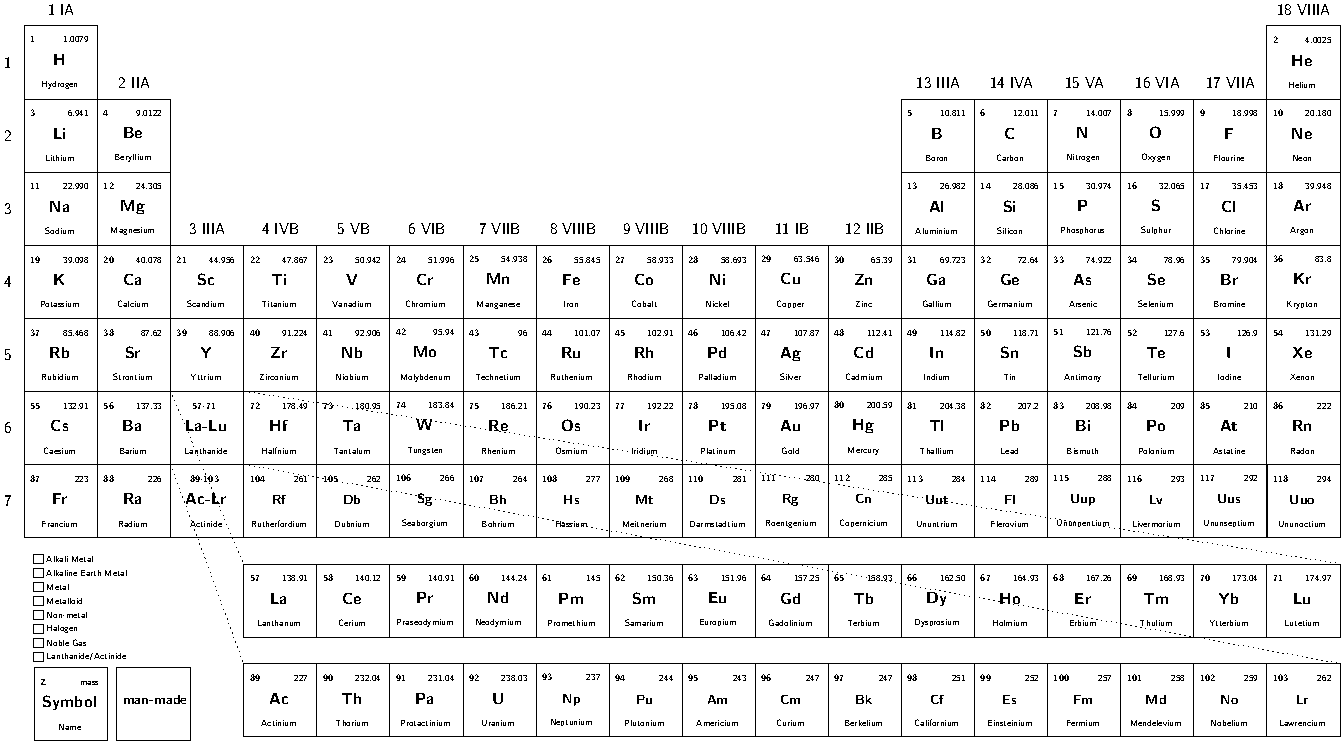
\includepdf[scale=0.7,angle=-90,pagecommand={\thispagestyle{fancy}}]{../codes/PeriodicTable/main.pdf}

%\section{Java}
%\subsection{Java Cheat Sheet}
%\lstinputlisting[language=java]{../codes/Java/Java_Cheat_Sheet.java}

\end{document}
